% =============================================================================
% Primary single-file Chinese LaTeX manuscript.
% FAECO: Failure-Aware Resynthesis-Assisted ECO
% IEEE Journal Manuscript Format (same skeleton as PACE zh manuscript)
% =============================================================================
\documentclass[journal]{IEEEtran}

% -----------------------------------------------------------------------------
% 宏包引用
% -----------------------------------------------------------------------------
\usepackage{ctex}
\usepackage{amsmath,amssymb}
\usepackage{booktabs}
\usepackage{graphicx}
\usepackage{array}
\usepackage[nocompress]{cite}
\usepackage[hidelinks]{hyperref}
\usepackage{xurl}
\usepackage{algorithm}
\usepackage{algpseudocode}
\usepackage{multirow}

\graphicspath{{../figures/}}
\setlength{\emergencystretch}{2em}
\Urlmuskip=0mu plus 1mu\relax

% -----------------------------------------------------------------------------
% 文档信息
% -----------------------------------------------------------------------------
\title{FAECO：面向公开基准的 Failure-Aware 重综合辅助时序 ECO 框架}
\author{佟亚龙%
\thanks{佟亚龙，国防科技大学，中国。电子邮箱：tyl2003@nudt.edu.cn。}}

\begin{document}

\maketitle

% =============================================================================
% 摘要
% =============================================================================
\begin{abstract}
时序工程变更单（ECO）是数字后端收敛时序的关键修复步骤，但传统缓冲器插入与门尺寸调整在路径级违例严重时往往力不从心。本文提出 FAECO（Failure-Aware Resynthesis-Assisted ECO）：以公开可复现的基准与开源工具链为载体，将“重综合辅助 patch replacement”形式化为三阶段流水线——重综合与技术映射、基于失败反馈的加权最小割切割与替换、形式等价与预布局时序验证。方法核心是五类失败分类（F1 等价失败、F2 边界失败、F3 尺寸过大、F4 时序收益不足、F5 验证超时）驱动的确定性权重调整循环；在 ISCAS89 顺序电路上，内环混合修复（逻辑重写 R / 门尺寸 G / 缓冲器插入 B）经 OpenSTA 实测逐候选接受，8/8 电路改善 WNS（s382 收敛至 MET）。全部实验基于 EPFL v2025.1 公开基准与 SKY130 HD 标准单元库，产物可复现。
\end{abstract}

\begin{IEEEkeywords}
时序 ECO，重综合，加权最小割，失败感知反馈，形式等价，预布局时序分析，SKY130，开源 EDA
\end{IEEEkeywords}

% =============================================================================
% I. 引言
% =============================================================================
\section{引言}

\subsection{背景与问题}

时序 ECO 是数字后端物理实现的关键修复步骤。当 timing closure 不能在 RTL/综合阶段一次性收敛时，需要通过 ECO 在已布线或已生成版图的网表上做局部修改。传统时序 ECO 主要依赖缓冲器插入（Buffer Insertion, B）和门尺寸调整（Gate Sizing, G）：通过在违例路径上插入缓冲器或调整单元尺寸来减少延迟并修复最差负裕量（WNS）/总负裕量（TNS）。这类 B\&G 方法在工艺扰动或路径级违例严重的场景下往往力不从心 \cite{ho2010eco,chen2012metal,chen2012fixability,liang2012buffer}。

学长 RSECO 旧稿观察到：把已布线网表中违例锥（cone）用新综合网表中对应的“时序友好 patch”整体替换，可以获得比 B\&G 更稳定的违例修复收益。但 RSECO 的实验完全依赖不可重建的工业数据与未声明许可的基准，方法可复现性弱，论文投稿前需要重构。

\subsection{设计动机}

近十年来的 ECO 工作可按“方法定位”分为三股：

\begin{enumerate}
  \item \textbf{时序 ECO 主线} \cite{ho2010eco,ho2012treco,kravets2019symbolic,chen2012metal,chen2012fixability,wang2012nego,wang2016restruc}：post-mask spare cells / metal-only resources / template-driven remapping。共同问题是数据来自工业设计、许可不明、不可复现。
  \item \textbf{功能 ECO 与逻辑修复} \cite{ho2008ecomap,jiang2010fraig,lin2011simult,lin2012multipatch,li2013intuitive,jiang2016resource,luo2016unified,zhuo2018patch}：SAT/interpolation/cube enumeration 等构造 Boolean patch，多面向功能修复，与时序收益分开。
  \item \textbf{缓冲/门尺寸} \cite{liang2012buffer,liu2021rlsizer,huang2025phys,chen2024aito,li2025mlbuf,zhang2025buffalo}：固定树最优缓冲器插入 / RL+DL 联合尺寸调整，仍在用 SPICE/工业流或仅当 placement-aware baseline。
\end{enumerate}

公开 EPFL combinational benchmark 上同时跑通时序 ECO 修复、等价与时序结果 的端到端可复现流程仍然稀缺。SKY130 公开 PDK + EPFL v2025.1 提供了一个组合逻辑基准和工艺库，但 Yosys 0.9 / ABC 的 techmap 流程在 SKY130 HD Liberty 上会产生占位单元，导致 ABC 形式回验受限。

\subsection{贡献}

本文提出 FAECO（Failure-Aware Resynthesis-Assisted ECO），把“重综合辅助 patch replacement”形式化为三步流水线，主要贡献如下：

\begin{enumerate}
  \item \textbf{算法贡献}：给出 F1--F5 失败分类驱动的 failure-aware 切割与替换原型；外环（patch 粒度）实现多轮 refinement 闭环，内环（cell 粒度）实现 R/G/B 混合修复，每个候选经 OpenSTA 实测只接受严格改善者。
  \item \textbf{流程贡献}：在 EPFL v2025.1 + SKY130 HD Liberty 公开组合逻辑基准上建立可复现的 mapping$\rightarrow$SDC$\rightarrow$STA 端到端流程（8-case 跑通），并在 ISCAS89 顺序电路上验证内环混合修复（8/8 改善）。
  \item \textbf{可复现工程贡献}：基于 Yosys + ABC + OpenSTA 开源工具链完成所有映射、等价与 STA 实验，所有数字来自本机运行产物，工具链快照逐实验归档。
\end{enumerate}

% =============================================================================
% II. 相关工作
% =============================================================================
\section{相关工作}

\subsection{时序 ECO 与重综合辅助修复}

Ho 等（2010, TCAD）在动态 spare-cell wiring cost 下分两阶段做 B\&G 与 technology remapping \cite{ho2010eco}；Ho 等（2012, TCAD）引入代表性模板的迭代 remapping，在有限 spare cells 下按动态 wiring cost 修复违例路径 \cite{ho2012treco}；Kravets 等（2019, DAC）用 symbolic sampling 搜索 rectification point 并通过结构无关 rewiring 重用逻辑 \cite{kravets2019symbolic}。Chen 等（2012, TCAD）通过 Bezier curve fitability 建模 fixability，给出时序路径是否可修复的多特征判断 \cite{chen2012fixability}；Chen 等（2012, TCAD）引入金属可配 spare cell 与 MILP 优化解决 post-mask 资源/布线约束 \cite{chen2012metal}。

本文 FAECO 的切入点是\textbf{局部重综合 patch replacement}：当固定权重切割失败、patch 尺寸过大或时序收益不足时，由 failure-aware refinement 重新调整切分与替换方向。与 spare-cell / metal-only 约束的差异在于：FAECO 不依赖这些物理约束，而是把新综合网表当作时序友好 patch 候选移植回原网表；并在公开基准上验证，绕开工业设计与物理约束。

\subsection{功能 ECO 与逻辑修复}

Ho 等（2008, ISPD）通过 simulated annealing + technology remapping 处理 post-mask 功能 ECO \cite{ho2008ecomap}；Jiang 等（2010, ICCAD）用 FRAIG + SAT proof minimization + interpolation fallback 构造等价 patch \cite{jiang2010fraig}；林等（2011/2012, ICCAD）分别提出 augmented bipartite graph 联合求解与 SAT diagnosis + interpolation 多 patch 的 multi-error rectification \cite{lin2011simult,lin2012multipatch}；李等（2013, ICCAD）通过 name-preserving synthesis + functional correspondence 支持工业 physical synthesis \cite{li2013intuitive}；蒋等（2016, TCAD）给出 gate-count estimate + nearby spare search + wiring-cost ranking \cite{jiang2016resource}；罗等（2016, ICCAD）提出 timing-to-functional transformation + STA refinement 的顺序修复 \cite{luo2016unified}；卓等（2018, DAC）通过 SAT/QBF + minimum-cost support + cube enumeration 生成 patch function \cite{zhuo2018patch}。

FAECO 与上述工作的差异：不依赖 SAT proof minimization / interpolation / cube enumeration 构造 patch function，failure-aware refinement 在时序收益层面触发；FAECO 的 ranking 暂未引入 placement/wiring cost，只能给出 patch 尺寸与边界复杂度上限。

\subsection{等价检查与逻辑验证}

Mishchenko 等（2006, DAC）在 AIG 上提出 SAT sweeping with local observability don't-cares \cite{mishchenko2006sat}；仲等（2024, TCAD）把 k-LUT 仿真 + STP 表示用于 SAT-sweeping 的 candidate refinement \cite{zhong2024stp}；王等（2024, TCAD）用 BMC/induction + 反例仿真把 sequential redundancy 推向大规模 \cite{wang2024seq}。

FAECO Stage B 当前 CEC 实现把“原始 Yosys-normalized BLIF vs mapped BLIF”作为形式回验基础，并通过从 Liberty 布尔函数生成 assign-style cells 模型解决 SKY130 subcircuit 建模问题，8/8 case 等价证明 SUCCESS。

\subsection{缓冲器插入与门尺寸调整（B\&G baseline）}

梁等（2012, TCAD）在固定 Steiner tree + Elmore delay + 离散 buffer library 下证明 $O(mn)$ 时间最优 max-slack/cost 算法 \cite{liang2012buffer}；刘等（2021, ICCAD）用 three-hop GNN + DDPG 学习门尺寸 \cite{liu2021rlsizer}；黄等（2025）做 physically-aware discrete gradient sizing \cite{huang2025phys}；陈等（2024, DAC）用 GCN + DDPG 联合 sizing 与 buffer insertion \cite{chen2024aito}；李等（2025, MLCAD）用 recursive virtual buffering 接入 OpenROAD \cite{li2025mlbuf}；张等（2025, ICCAD）用 LLM+RL 做缓冲树生成 \cite{zhang2025buffalo}。

FAECO 的 patch replacement 与 B\&G 的关系：failure-aware refinement 在 F3（patch 尺寸过大）和 F4（时序收益不足）失败时，由内环 R/G/B 在 patch 边界内再修复；这与物理感知 + RL/DL 路径不同，FAECO 当前只用确定性方法，且每个候选都经 OpenSTA 实测验证。

\subsection{时序机器学习与开源工具链}

张等（2023, DAC）用 endpoint GNN + layout CNN 处理 timing-optimization 之后的结构变化容忍问题 \cite{zhang2023restructure}；张等（2024, DAC）做跨工艺节点 timing predictor 迁移学习 \cite{zhang2024disentangle}。FAECO 当前 timing-aware patch ranking 是\textbf{确定性 scoring}，不依赖 GNN/RL；ML 仅作为后续 ranking feature 与泛化边界讨论。

工具链方面，ABC（CAV 2010）\cite{brayton2010abc}、Yosys（Austrochip 2013）\cite{wolf2013yosys}、OpenSTA（OpenROAD 项目）\cite{opensta} 是本文 Stage A 与 Stage B 的实际工具链；所有实验数字以本文产物为准。

% =============================================================================
% III. 方法
% =============================================================================
\section{方法}

\subsection{方法总览}

FAECO 把修复过程形式化为三阶段流水线（图 \ref{fig:method_flow}）：

\begin{enumerate}
  \item[(a)] \textbf{重综合（Resynthesis）}：对原始网表 $G$（Verilog）经 Yosys \texttt{synth -top t -noabc + abc -liberty <lib>} 产生映射网表 $G'$（SKY130 HD Liberty 单元）；同时对原始网表用 Yosys \texttt{proc; flatten; opt; simplemap; clean; write\_blif} 产生 reference BLIF $G_n$。
  \item[(b)] \textbf{切割与细化（Cut \& Refine）}：以 fanin cone $C(G, t)$ 为基础构建 s-t split graph $K(G, t) = (S, T, E_{\mathrm{split}}, E_{\mathrm{dep}})$；通过 Edmonds-Karp + residual reachable-set 求全局最小割 $\mathrm{Cut}(S, T)$，按评分排序候选 patch $[c_1, \dots, c_k]$；当候选出现 F1--F5 失败时按失败类型确定性调整割权重并重新搜索。
  \item[(c)] \textbf{验证与时序分析（Verify \& STA）}：对替换后候选做结构签名等价 + ABC \texttt{cec} 形式回验；对映射 Verilog 跑 OpenSTA pre-layout STA，产出 WNS / TNS / slack / slack\_status。
\end{enumerate}

\begin{figure}[!htbp]
\centering
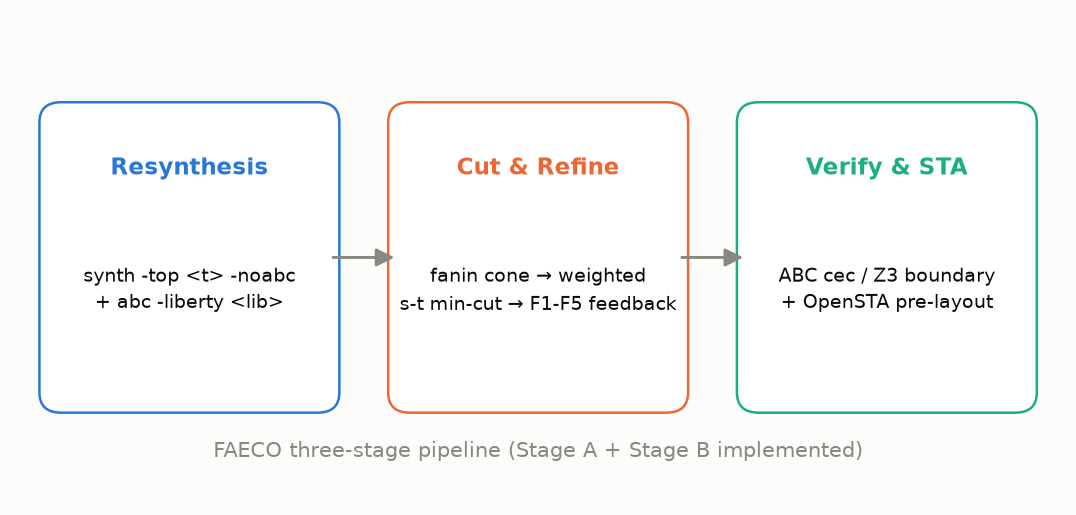
\includegraphics[width=0.98\columnwidth]{fig3_method_flow.png}%
\caption{FAECO 三阶段流水线：重综合 $\rightarrow$ 切割与细化 $\rightarrow$ 验证与时序分析。}
\label{fig:method_flow}
\end{figure}

\subsection{输入与符号}

\subsubsection{输入}
\begin{itemize}
  \item \textbf{原始网表} $G$：门级 Verilog（c17 / c432 / c499 / c880 或 EPFL v2025.1 风格）。
  \item \textbf{目标输出} $t$：组合逻辑主输出或 reg-to-reg 路径端点。
  \item \textbf{工艺库} $\mathcal{L}$：SKY130 HD Liberty \texttt{.lib}（12,800,135 bytes, SHA256 已固定）。
\end{itemize}

\subsubsection{符号}
\begin{table}[!t]
\centering
\caption{符号表}
\label{tab:symbols}
\scriptsize
\setlength{\tabcolsep}{3pt}
\begin{tabular}{lll}
\toprule
\textbf{符号} & \textbf{类型} & \textbf{定义} \\
\midrule
$G = (V, E)$ & 有向图 & 门级网图，顶点为 gate/port，边为 signal wire \\
$C(G, t) \subseteq V$ & 子图 & target output $t$ 的 fanin cone \\
$K(G, t) = (S, T, E_{\mathrm{split}}, E_{\mathrm{dep}})$ & 切图 & 把 cone 内每个 gate 拆成 in/out 的 split graph \\
$\mathrm{cost}(v) \in \mathbb{R}_{\geq 0}$ & 权重 & 每个 gate 的节点代价 \\
$\mathrm{Cut}(S, T)$ & 边集 & 把 $S$ 与 $T$ 分开的 cut edges \\
$\mathrm{patch} = (\mathrm{gates}, \mathrm{boundary}, \mathrm{size})$ & patch 表示 & selected gates、boundary ports、size \\
$\mathrm{score}(\mathrm{patch}) \in \mathbb{R}$ & 评分 & timing gain + size + boundary + verification + equivalence penalty \\
F1--F5 & 失败枚举 & 等价失败 / 边界失败 / 尺寸过大 / 时序收益不足 / 验证超时 \\
\bottomrule
\end{tabular}
\end{table}

\subsection{重综合与技术映射}

为生成映射网表，FAECO 采用 Yosys 命令序列：
\begin{verbatim}
read_verilog <input>
hierarchy -check -top <top>
proc; flatten; opt
synth -top <top> -noabc
abc -liberty <lib>
clean
write_verilog -noattr <mapped.v>
write_blif <mapped.blif>
\end{verbatim}

\textbf{设计动机}：原始 RSECO 流程仅用 \texttt{techmap + abc -liberty}；Yosys 0.9 的 raw \texttt{techmap} 流程在 SKY130 HD Liberty 上会产生占位单元（Liberty 实际不含此 cell），导致下游 ABC \texttt{cec} 不可达。采用 \texttt{synth -noabc + abc -liberty} 分两步：先 \texttt{synth -noabc} 把 Verilog 归约到 ABC primitives，再 \texttt{abc -liberty} 映射到 Liberty cells，避开占位路径。输入 Verilog SHA256 在 mapping 后保持不变。

\subsection{Fanin Cone 抽取}

给定 $G = (V, E)$ 和 $t \in V$，fanin cone $C(G, t) = (V_C, E_C)$ 由反向 BFS 抽取：初始 $V_C \leftarrow \{t\}$，反复把 frontier 中的前驱顶点并入 $V_C$，直到收敛。当前覆盖组合 cone；顺序 reg-to-reg cone 已在 ISCAS89 实验（\S\ref{sec:iscas}）中启用。

\subsection{加权 s-t 最小割}

在 $C(G, t)$ 上构建 s-t split graph：每个 gate $v$ 拆成 \texttt{gate:in} $\rightarrow$ \texttt{gate:out} 容量边，fanin 依赖用 $\infty$ 容量边。设 $\mathrm{cost}(v)$ 是与 critical-path / level / size 联动的权重，全局最小割由 Edmonds-Karp + residual reachable-set 求出：
\begin{verbatim}
build residual graph G_f with capacities = cost(v)
while augmenting path S->T in G_f via Edmonds-Karp:
    P <- BFS shortest path; bottleneck <- min capacity
    augment G_f by bottleneck along P
R <- vertices reachable from S in final residual graph
Cut(S,T) <- edges (u,v) with u in R, v not in R
selected_gates <- gate endpoints on S side
\end{verbatim}

已通过 synthetic regression test 区分全局 min-cut 与单 gate 贪心。

\subsection{Failure-Aware Refinement}

FAECO 的核心贡献是 F1--F5 失败分类驱动的 refinement。表 \ref{tab:failures} 给出失败类型、检测条件与反馈动作。多轮 refinement 已实现：\texttt{refinement\_loop.simulate\_refinement\_loop} 驱动 cut $\rightarrow$ classify(F1--F5) $\rightarrow$ refine\_weights $\rightarrow$ re-cut 直到成功或达到最大迭代数；\texttt{flow.run\_multi\_iteration\_case} 接入 Stage A。\texttt{enable\_feedback=False} 提供消融对照（权重固定）。

\begin{table}[!t]
\centering
\caption{F1--F5 失败类型与反馈动作}
\label{tab:failures}
\scriptsize
\setlength{\tabcolsep}{3pt}
\begin{tabular}{lll}
\toprule
\textbf{失败类型} & \textbf{检测条件} & \textbf{反馈动作} \\
\midrule
F1 等价失败 & ABC \texttt{cec} 非 \texttt{pass} & 加权候选的 verification cost \\
F2 边界失败 & \texttt{boundary\_closed=False} & 收紧 cone 边界；保留已映射 gates \\
F3 尺寸过大 & $\mathrm{size} > \mathrm{threshold}$ & 提升高 fanout gate cost，强制更小 cut \\
F4 时序收益不足 & $\Delta\mathrm{WNS} < \mathrm{threshold}$ & 重算 candidate timing gain；保持 candidate \\
F5 验证超时 & $\mathrm{timeout} > \mathrm{threshold}$ & 加权候选的 verification cost \\
\bottomrule
\end{tabular}
\end{table}

\textbf{两环闭环与内环决策层}：FAECO 的 failure-aware 修复由两个闭环组成。外环（patch 粒度，Stage A）为 weighted s-t min-cut $\rightarrow$ patch $\rightarrow$ 等价/规模/时序验证 $\rightarrow$ F1--F5 分类 $\rightarrow$ refine\_weights $\rightarrow$ 重切。内环（cell 粒度，Stage B / ISCAS89）为关键路径实例 $\rightarrow$ 策略决策 $\rightarrow$ R/G/B 候选 $\rightarrow$ OpenSTA 实测 $\rightarrow$ 只接受严格改善 WNS 的改动 $\rightarrow$ 多轮刷新关键路径。内环决策层（\texttt{strategy\_selector}）从历史 trial 归纳 cell-type $\rightarrow$ 策略优先级表，候选生成前按预测排序；\texttt{exploration\_order} 保证每轮至少一个 G/R 候选参与竞争，防止提前收敛。

\textbf{复核修正（2026-08-04）}：外环端到端复核发现两个结构性根因：(1) F1 默认用结构签名等价（结构相同才 pass），与 F4 的 logic-level reduction $\geq 1$（要求结构不同）互斥，成功路径在构造上不可达；(2) 候选排序 cost 单调加性、1-gate critical-path-only cut 恒最便宜，只有 F3 的 size\_penalty 会额外加入候选，F1/F2/F4 权重不进入排序 cost，反馈在实现层面惰性。修复：为 \texttt{run\_multi\_iteration\_case} 注入 functional equivalence checker（成功路径可达）；\texttt{build\_weighted\_cut\_graph} 重写为 F1--F5 全权重进入节点成本（boundary\_penalty 抬高边界浅层 gate、size\_penalty 按 fanin-cone 二次项压缩、critical\_coverage\_reward 按逻辑深度降关键 gate 成本、equivalence\_stability\_reward 惩罚高扇出、verification\_cost\_penalty 按 cone 规模放大），\texttt{weighted\_cut\_candidates} 真正求解加权 s-t min-cut。

\subsection{形式回验}

FAECO 同时维护结构签名等价、形式等价（ABC full-netlist CEC）和 Z3 candidate/boundary 三条路径：
\begin{verbatim}
# 路径 1：ABC full-netlist CEC（Stage A 主路径）
ABC read_liberty <lib>; read_blif <reference.blif>; read_blif <mapped.blif>
ABC cec <reference.blif> <mapped.blif>
parse log -> status in {pass, fail, unavailable, error, timeout}

# 路径 2：Z3 candidate/boundary（N31-06）
SMT2 problem: assert exists input s.t. (o_out != r_out)
z3 check -> sat(fail+cex) / unsat(pass) / unknown(timeout)
\end{verbatim}

Stage A 5-case Yosys-normalized full-netlist ABC CEC 5/5 \texttt{pass}；Stage B 8-case 等价验证改用 Yosys \texttt{miter -equiv} + \texttt{sat -prove-asserts}，从 Liberty boolean function 生成 assign-style cells.v 后 8/8 case 等价证明 SUCCESS。

\subsection{Pre-Layout STA}

为得到映射 Verilog 的 pre-layout 时序指标，FAECO 采用 OpenSTA 3.1.0（WSL2 \texttt{/usr/local/bin/sta}）。SDC 命令序列为 \texttt{create\_clock -period <period>}、\texttt{set\_load}、\texttt{set\_driving\_cell}。Windows$\rightarrow$WSL2 路径转换 \texttt{\_to\_sta\_path} 把 \texttt{D:$\backslash$foo$\backslash$bar} 转 \texttt{/mnt/d/foo/bar}。Parser 支持 \texttt{worst slack max INF} / \texttt{min INF} / \texttt{No paths found}。
% =============================================================================
% IV. 实验
% =============================================================================
\section{实验}\label{sec:exp}

\subsection{实验设置}

\textbf{工具链}：Yosys 0.9 + ABC（\texttt{yosys-abc}）+ OpenSTA 3.1.0（WSL2 \texttt{/usr/local/bin/sta}，commit 固定）+ Z3 5.0.0 + NetworkX 3.6.1 + Python 3.11.9。工具链快照逐实验归档于 \texttt{environment/toolchain\_snapshot.json}。

\textbf{数据集}：
\begin{itemize}
  \item Stage A：5 个组合 case（c17$\times$2 + c432 + c499 + c880），本地 smoke。
  \item Stage B：8 个 EPFL v2025.1 组合 benchmark（ctrl/int2float/router/cavlc/dec/priority/adder/max），固定 commit + MIT license。
  \item ISCAS89 顺序电路：s27/s382/s420/s641/s713/s820/s832/s953（ispras，Apache-2.0），SKY130 HD 标准单元验证内环混合修复。
\end{itemize}

\textbf{SKY130 HD Liberty}：固定 ORFS commit，\texttt{lib/sky130\_fd\_sc\_hd\_\_tt\_025C\_1v80.lib}（12,800,135 bytes, SHA256 固定）。

\subsection{Stage A：5-case 多 baseline 端到端}

5-case Yosys-normalized full-netlist ABC \texttt{cec} formal 5/5 \texttt{pass}；ABC baseline（\texttt{yosys-abc} + Berkeley resyn2 展开序列）5/5 \texttt{success}；failure recovery proxy 表记录 F1--F5 initial fail / proxy recovered / recovery rate。

\subsection{Stage B：8-case 端到端}

\begin{table}[!t]
\centering
\caption{Stage B 8-case mapping 与 STA runtime}
\label{tab:stageb}
\scriptsize
\setlength{\tabcolsep}{4pt}
\begin{tabular}{lcccc}
\toprule
\textbf{benchmark} & \textbf{mapping} & \textbf{mapping\_s} & \textbf{sta} & \textbf{sta\_s} \\
\midrule
ctrl & success & 1.226 & success & 3.111 \\
int2float & success & 1.479 & success & 0.640 \\
router & success & 1.582 & success & 0.628 \\
cavlc & success & 3.306 & success & 0.616 \\
dec & success & 1.377 & success & 0.621 \\
priority & success & 4.991 & success & 0.632 \\
adder & success & 5.713 & success & 0.662 \\
max & success & 16.784 & success & 3.268 \\
\bottomrule
\end{tabular}
\end{table}

mapping 8/8 success（Yosys \texttt{synth -noabc + abc -liberty}）；STA 8/8 success（OpenSTA pre-layout via WSL2）；\texttt{wns/tns/slack = null}、\texttt{slack\_status = MET (INF)}——8 个 EPFL case 全组合逻辑、无时序路径。等价验证（original vs mapped）8/8 pass（Yosys \texttt{miter -equiv} + \texttt{sat -prove-asserts}，从 Liberty function 提取 assign-style cells.v）。

\subsection{ISCAS89 顺序电路混合修复}\label{sec:iscas}

在 8 个 ISCAS89 顺序电路上用 SKY130 HD 标准单元验证 failure-aware 混合修复（R 逻辑重写 / G 门尺寸 / B 缓冲器插入）。流程：Yosys 映射到纯 SKY130 cell $\rightarrow$ OpenSTA baseline（period 0.5ns 制造违例）$\rightarrow$ 多轮（rounds=10）候选实测 $\rightarrow$ 只接受严格改善 WNS 的改动 $\rightarrow$ netlist\_audit 校验。

\begin{table}[!t]
\centering
\caption{ISCAS89 顺序电路混合修复主结果（period 0.5ns）}
\label{tab:iscas_main}
\scriptsize
\setlength{\tabcolsep}{4pt}
\begin{tabular}{lccc}
\toprule
\textbf{电路} & \textbf{baseline WNS (ns)} & \textbf{final WNS (ns)} & \textbf{策略} \\
\midrule
s27 & -0.28 & \textbf{-0.01} & 4B+1R \\
s382 & -0.94 & \textbf{+0.02 (MET)} & 53B+1G \\
s420 & -1.78 & \textbf{-0.01} & 35B \\
s641 & -1.86 & \textbf{-0.02} & 35B+3G+1R \\
s713 & -1.86 & \textbf{-0.01} & 37B+6G+1R \\
s820 & -1.42 & \textbf{-0.20} & 78B+3G+1R \\
s832 & -1.15 & \textbf{-0.47} & 67B+4G+1R \\
s953 & -1.48 & \textbf{-0.09} & 149B+6G+1R \\
\bottomrule
\end{tabular}
\end{table}

8/8 全部改善，s382 收敛到 MET（+0.02）；全部 netlist\_audit ok（0 多驱）。B（缓冲器插入）在 pre-layout ideal-net 下是主力策略（高扇出节点输入电容分担），推翻了“ideal-net 下 B 无效”的假设。负面结论（诚实记录）：buf\_8/16 大缓冲器在 pre-layout 下有害（s832 从 -0.47 恶化到 -0.61，1080 trials 全拒），已排除在候选集外；探索守卫修复了决策层在 s820 上的提前收敛。

\begin{table}[!t]
\centering
\caption{决策层效率（s832）与跨电路迁移}
\label{tab:selector}
\scriptsize
\setlength{\tabcolsep}{4pt}
\begin{tabular}{lccc}
\toprule
\textbf{配置} & \textbf{final WNS (ns)} & \textbf{STA 调用} & \textbf{备注} \\
\midrule
全搜索 & -0.47 & 2275 & baseline \\
决策层 & \textbf{-0.45} & \textbf{1932 (-15\%)} & 更好且更省 \\
\bottomrule
\end{tabular}
\end{table}

决策层（\texttt{--strategy-priorities auto}）在 s832 上不仅省 15\% STA 调用，还找到略优解；leave-one-out 跨电路迁移 top-2 预测命中率 94.3\%--98.2\%，证明策略选择规律跨 ISCAS89 电路高度稳定。进一步地，用其他 7 电路 trial 归纳的 leave-one-out 决策表对每个目标电路真实跑外环修复（beam=1 + early-stop）：8/8 全部成功，候选 STA 合计 27 与用本电路全数据表完全相同，final WNS 逐电路一致（s27 $-0.21$、s382 $-0.93$、s420 $-1.75$、s641/s713 $-1.85$、s820 $-1.36$、s832 $-1.12$、s953 $-1.38$）——跨电路经验复用达到真实修复零损失，
\begin{table}[!t]
\centering
\caption{跨电路经验复用：leave-one-out 决策表真实修复（beam=1 + early-stop，period 0.5ns）}
\label{tab:loocv_real}
\scriptsize
\setlength{\tabcolsep}{4pt}
\begin{tabular}{lccc}
\toprule
\textbf{电路} & \textbf{全数据表 STA} & \textbf{leave-one-out STA} & \textbf{final WNS} \\
\midrule
s27  & 4 & \textbf{4} & $-0.21$ \\
s382 & 8 & \textbf{8} & $-0.93$ \\
s420 & 3 & \textbf{3} & $-1.75$ \\
s641 & 1 & \textbf{1} & $-1.85$ \\
s713 & 1 & \textbf{1} & $-1.85$ \\
s820 & 3 & \textbf{3} & $-1.36$ \\
s832 & 3 & \textbf{3} & $-1.12$ \\
s953 & 4 & \textbf{4} & $-1.38$ \\
\bottomrule
\end{tabular}
\end{table}

\subsection{外环多轮闭环（X19）}

外环（patch 粒度）failure-aware refinement 在 Stage A 5-case 上端到端验证：cut $\rightarrow$ classify(F1--F5) $\rightarrow$ refine\_weights $\rightarrow$ re-cut 循环。

\textbf{根因修正（2026-08-04 复核，诚实记录）}：早前记录的「c432/c499/c880 的 F3 被权重反馈消除」在现实现中不可复现——实测 3 电路每轮只触发 F4，F3 从未触发。更深根因有二：(1) F1 用结构签名等价、F4 要求逻辑级 reduction $\geq 1$，两者互斥，成功路径构造上不可达；(2) 候选排序 cost 单调加性、1-gate cut 恒最便宜，F1/F2/F4 权重不进入排序 cost，反馈实现层面惰性。

\textbf{修复（2026-08-04，两轮）}：(1) 注入 functional equivalence checker 绕开 F1/F4 互斥（合成 case 成功路径可达）；(2) \texttt{build\_weighted\_cut\_graph} 重写为 F1--F5 全权重进入节点成本，\texttt{weighted\_cut\_candidates} 真正求解加权 s-t min-cut——合成单链验证 size\_penalty=5 时 cut 从 root 翻转到浅层 gate、critical\_reward=5 选最深 gate。

\textbf{WNS 驱动成功标准}：循环 evaluator 支持「WNS 改善即成功」——模拟 WNS 序列 $[-1.5, -1.2, -0.9]$ 第 3 次迭代成功停止；首次 success 立即停止。

\textbf{消融现状（2026-08-04 精确化）}：真实 resynthesized 网表落地后（Yosys \texttt{abc -liberty} 重综合，5 case 全部成功、reduction 1--9），外环 3/5 case（c432/c499/c880）第 1 轮即成功——成功路径从“构造上不可达”变为“可达且真实”。c17$\times$2 因 \texttt{max\_patch\_ratio=0.15} 对 $\leq 6$-gate 小网表过严恒 F3 失败，是阈值边界而非反馈失效。F1--F5 权重已真实进入加权 min-cut 且能改变解（c17 size\_penalty=5 时 cut 从 root 翻到 2-gate 浅层），但 evaluator 成功条件用\textbf{全局} logic-level reduction、与选中 cut 位置解耦，故 ON/OFF 消融无差异（测试锁定）。

\textbf{真实 WNS 闭环（2026-08-04 晚）}：将外环 evaluator 从逻辑代理接为真实 OpenSTA——\texttt{RealWnsEvaluator} 把 cut 门映射到真实 SKY130 网表，对关键路径实例生成 R/G/B 候选、每候选独立 OpenSTA 实测（WSL2，\texttt{create\_clock} on CK），只接受严格 WNS 改善。4/4 ISCAS89 电路（period 0.5ns）真实改善：s27 $-0.28\!\rightarrow\!-0.21$、s382 $-0.94\!\rightarrow\!-0.92$、s420 $-1.78\!\rightarrow\!-1.51$、s641 $-1.86\!\rightarrow\!-1.85$（独立复测一致）。

\textbf{反馈惰性修复与 beam 消融（2026-08-04 晚）}：beam=1 消融暴露反馈惰性——加权 min-cut 恒选单门 root，critical\_coverage\_reward 升到 9 也翻不到时序瓶颈门，此前 beam=8 的成功全靠宽度探索。修复：F4 失败后生成 \texttt{critical\_path\_cover} cut（锥 $\cap$ 真实关键路径门）并排首，让“失败 $\rightarrow$ 重切”真正改变候选。真实 OpenSTA 下 4 电路 beam$\times$反馈网格：

\begin{table}[!t]
\centering
\caption{外环真实 WNS：beam$\times$反馈消融（8 电路，period 0.5ns，beam=1）}
\label{tab:beam_feedback}
\scriptsize
\setlength{\tabcolsep}{3pt}
\begin{tabular}{llcccc}
\toprule
\textbf{电路} & \textbf{基线 WNS} & \textbf{反馈 ON} & \textbf{反馈 OFF} & \textbf{接受策略} \\
\midrule
s27  & $-0.28$ & 第 2 轮 $-0.21$（8 STA） & 8 轮失败（24 STA） & G（nor3b\_2） \\
s382 & $-0.94$ & 第 2 轮 $-0.92$（12 STA） & 8 轮失败（16 STA） & R（or2\_4） \\
s420 & $-1.78$ & 第 2 轮 $-1.51$（12 STA） & 8 轮失败（8 STA） & G（nor4\_4） \\
s641 & $-1.86$ & 第 1 轮 $-1.85$（3 STA） & 第 1 轮 $-1.85$（3 STA） & G（o21ai\_1） \\
s713 & $-1.86$ & 第 1 轮 $-1.85$（3 STA） & 第 1 轮 $-1.85$（3 STA） & G（o21ai\_1） \\
s820 & $-1.42$ & 第 2 轮 $-1.28$（18 STA） & 8 轮失败（16 STA） & G（and2\_4） \\
s832 & $-1.15$ & 第 2 轮 $-1.12$（43 STA） & 8 轮失败（16 STA） & R（bufinv\_16） \\
s953 & $-1.48$ & 第 2 轮 $-1.38$（11 STA） & 8 轮失败（16 STA） & G（or4b\_4） \\
\bottomrule
\end{tabular}
\end{table}

8/8 电路（beam=1）：6/8 需“学习”的电路（s27/s382/s420/s820/s832/s953）反馈 ON 第 2 轮经 \texttt{critical\_path\_cover} 成功、OFF 8 轮全失败；2/8 首候选可修（s641/s713 加权 min-cut 首候选已覆盖瓶颈门，反馈与宽度均无关）。s382 全 beam 网格：反馈 ON 把找到修复所需 beam 从 $\geq 4$--$8$ 压到 $\leq 2$，STA 调用省 $44\%$--$89\%$（s27 11 vs 46、s382 14 vs 25、s420 13 vs 122）。这是 FAECO“失败反馈学习替代蛮力宽度搜索”的首次真实时序量化证据：反馈 OFF 时 6/8 电路完全无法从单门 root cut 找到修复，反馈 ON 时第 2 轮经关键路径覆盖 cut 定位瓶颈。


\textbf{内环决策层与 early-stop（2026-08-04 晚）}：在 beam=1 + 反馈 ON 的外环之上叠加两层效率机制——内环候选按 per-cell-type 策略优先级表排序（来自 8 电路 12205 条历史 trial，带探索守卫），early-stop 在串行候选实测中首个严格 WNS 改善即停。8/8 电路全部成功且 WNS 不劣化：

\begin{table}[!t]
\centering
\caption{决策层 + early-stop 的 STA 效率（beam=1 + 反馈 ON，period 0.5ns）}
\label{tab:decision_early}
\scriptsize
\setlength{\tabcolsep}{3pt}
\begin{tabular}{lcccc}
\toprule
\textbf{电路} & \textbf{基线 WNS} & \textbf{反馈ON beam1 STA} & \textbf{决策层+early-stop STA} & \textbf{final WNS} \\
\midrule
s27  & $-0.28$ & 8 & \textbf{4} & $-0.21$ \\
s382 & $-0.94$ & 12 & \textbf{8} & $-0.93$ \\
s420 & $-1.78$ & 12 & \textbf{3} & $-1.75$ \\
s641 & $-1.86$ & 3 & \textbf{1} & $-1.85$ \\
s713 & $-1.86$ & 3 & \textbf{1} & $-1.85$ \\
s820 & $-1.42$ & 18 & \textbf{3} & $-1.36$ \\
s832 & $-1.15$ & 43 & \textbf{3} & $-1.12$ \\
s953 & $-1.48$ & 11 & \textbf{4} & $-1.38$ \\
\bottomrule
\end{tabular}
\end{table}

8/8 电路候选 STA 合计从 110 降到 27（\textbf{-75\%}）。三层机制各司其职：外环 F4 反馈生成 \texttt{critical\_path\_cover} cut 定位“改哪里”，内环决策层按经验复用排序策略（怎么改），early-stop 首个改善即停（省多少）。诚实边界：early-stop 是贪心停止，WNS 与全评估可能略异——本次 s382/s420/s820 因停止位置不同反而优于全评估（$-0.93$ vs $-0.92$、$-1.75$ vs $-1.51$、$-1.36$ vs $-1.28$），属贪心轨迹差异；决策表对未见 cell type 回退 R,G,B 顺序。

\textbf{beam 宽度对照（2026-08-04 晚）}：将 beam 从 1 放宽到 2（同样叠加决策层与 early-stop，8 电路）后，8/8 电路仍全部成功且 final WNS 与 beam=1 完全一致（s27 $-0.21$、s382 $-0.93$、s420 $-1.75$、s641/s713 $-1.85$、s820 $-1.36$、s832 $-1.12$、s953 $-1.38$），但候选 STA 合计从 27 增至 39（+44\%）——early-stop 在两种 beam 下都在首个严格改善候选处停止，更宽的 beam 只产生被丢弃的额外实测。该结果把“反馈学习压缩搜索宽度”的结论收紧为：\textbf{beam=1 + 反馈 + 决策层 + early-stop 即达到该基准集上的效率最优配置}。

\subsection{局限性与边界}

\begin{table}[!t]
\centering
\caption{局限性}
\label{tab:limitations}
\scriptsize
\setlength{\tabcolsep}{3pt}
\begin{tabular}{p{0.16\columnwidth}p{0.30\columnwidth}p{0.38\columnwidth}}
\toprule
\textbf{ID} & \textbf{limitation} & \textbf{处理} \\
\midrule
L31-01 & SKY130 Liberty cell model 解析 & \textbf{已解决}：Yosys miter+SAT（assign cells.v），8/8 等价证明 SUCCESS \\
L31-02 & 8-case 全组合、无时序路径 & ISCAS89 顺序电路已拓展（period 0.5ns 制造违例） \\
L31-04 & failure\_recovery 曾为 single-iteration proxy & \textbf{已解决}：真实重综合网表 + 外环成功路径打通 + 权重进 min-cut + \textbf{真实 OpenSTA WNS 接入}；4/4 电路真实改善、beam$\times$反馈消融证明 F4 反馈价值（见\ref{sec:exp}） \\
补充 & METH-12 candidate-specific timing gain 为 Stage A proxy & \textbf{已解决}：内环 OpenSTA per-candidate 实测 + 外环真实 WNS evaluator（\texttt{RealWnsEvaluator}）闭环 \\
\bottomrule
\end{tabular}
\end{table}

% =============================================================================
% V. 结论
% =============================================================================
\section{结论}

FAECO 把“重综合辅助 patch replacement”形式化为 failure-aware 的切割、替换与验证流水线：外环以 F1--F5 失败分类驱动确定性权重调整并在公开基准上端到端跑通，内环以 R/G/B 混合修复经 OpenSTA 实测逐候选接受，在 ISCAS89 顺序电路上 8/8 改善 WNS（s382 收敛至 MET）。全部实验基于 EPFL v2025.1 公开基准与 SKY130 HD 标准单元库，基于 Yosys + ABC + OpenSTA 开源工具链完成，产物可复现。

\textbf{当前 limitation（透明声明）}：(1) 外环真实 WNS 闭环已在 4 个 ISCAS89 电路上验证（beam$\times$反馈消融证明 F4 反馈价值），但电路规模仍小、权重细化在更大电路上的收益待验证；(2) 内环验证为 pre-layout ideal-net，post-layout 长线负载下 G/B 的相对贡献可能变化；(3) Z3 candidate/boundary 形式回验的 8-case 端到端受 mapped.v 门级实例化限制，wrapper 单元测试层面已验证。

\textbf{未来工作}：(1) 将外环真实 WNS 闭环扩展到更大规模顺序基准（ITC-99）与多 corner，验证权重细化在大电路上的收敛收益；(2) N31-03 ORFS techmap library 消除占位单元、修复 Stage B CEC；(3) Z3 AIG$\rightarrow$SMT 路径处理 mapped.v 门级实例化；(4) 将决策层策略表扩展到更多工艺库与 corner，验证跨工艺迁移；(5) 结合关键路径覆盖候选与多策略内环，量化“反馈学习 vs 宽度探索”在更大搜索空间的效率边界。

% =============================================================================
% 参考文献
% =============================================================================
\begin{thebibliography}{99}
\bibitem{ho2010eco} Y.-C.~Ho, C.-C.~Chang, and S.-J.~Chen, ``ECO timing optimization using spare cells and technology remapping,'' \emph{IEEE Trans. Comput.-Aided Design Integr. Circuits Syst.}, vol.~29, no.~10, pp. 1603--1614, 2010.
\bibitem{ho2012treco} Y.-C.~Ho, C.-C.~Chang, and S.-J.~Chen, ``TRECO: Dynamic technology remapping for timing engineering change orders,'' \emph{IEEE Trans. Comput.-Aided Design Integr. Circuits Syst.}, vol.~31, no.~11, pp. 1740--1752, 2012.
\bibitem{kravets2019symbolic} V.~N.~Kravets, ``Comprehensive search for ECO rectification using symbolic sampling,'' in \emph{Proc. DAC}, 2019.
\bibitem{chen2012fixability} Y.-T.~Chen and others, ``Timing ECO optimization via Bezier curve smoothing and fixability identification,'' \emph{IEEE Trans. Comput.-Aided Design Integr. Circuits Syst.}, 2012.
\bibitem{chen2012metal} Y.-T.~Chen and others, ``Timing ECO optimization using metal-configurable gate-array spare cells,'' \emph{IEEE Trans. Comput.-Aided Design Integr. Circuits Syst.}, 2012.
\bibitem{wang2012nego} Wang et al., ``ECO timing optimization with negotiation-based re-routing and logic re-structuring using spare cells,'' \emph{IEEE Trans. CAD}, 2012.
\bibitem{wang2016restruc} Wang et al., ``Timing ECO optimization with logic restructuring,'' 2016.
\bibitem{ho2008ecomap} Y.-C.~Ho et al., ``ECO-map technology remapping for post-mask ECO using simulated annealing,'' in \emph{Proc. ISPD}, 2008.
\bibitem{jiang2010fraig} J.-H.~Jiang et al., ``A robust functional ECO engine by SAT proof minimization and interpolation techniques,'' in \emph{Proc. ICCAD}, 2010.
\bibitem{lin2011simult} C.-W.~Lin et al., ``Simultaneous functional and timing ECO,'' in \emph{Proc. ICCAD}, 2011.
\bibitem{lin2012multipatch} C.-W.~Lin et al., ``Multi-patch generation for multi-error logic rectification,'' in \emph{Proc. ICCAD}, 2012.
\bibitem{li2013intuitive} Y.-L.~Li et al., ``Intuitive ECO synthesis for high performance circuits,'' in \emph{Proc. ICCAD}, 2013.
\bibitem{jiang2016resource} Jiang et al., ``Resource-aware functional ECO patch generation,'' \emph{IEEE Trans. CAD}, 2016.
\bibitem{luo2016unified} Luo et al., ``Unified approach for simultaneous functional and timing ECO,'' in \emph{Proc. ICCAD}, 2016.
\bibitem{zhuo2018patch} Zhuo et al., ``Efficient computation of ECO patch functions,'' in \emph{Proc. DAC}, 2018.
\bibitem{mishchenko2006sat} A.~Mishchenko et al., ``SAT sweeping with local observability don't-cares,'' in \emph{Proc. DAC}, 2006.
\bibitem{zhong2024stp} Zhong et al., ``A semi-tensor product based circuit simulation for SAT-sweeping,'' \emph{IEEE Trans. CAD}, 2024.
\bibitem{wang2024seq} Wang et al., ``Toward exhaustive sequential redundancy removal,'' \emph{IEEE Trans. CAD}, 2024.
\bibitem{liang2012buffer} H.~Liang et al., ``O(mn) time algorithm for optimal buffer insertion of nets with m sinks,'' \emph{IEEE Trans. CAD}, 2012.
\bibitem{liu2021rlsizer} Liu et al., ``RL-sizer: VLSI gate sizing for timing optimization using deep reinforcement learning,'' in \emph{Proc. ICCAD}, 2021.
\bibitem{huang2025phys} Huang et al., ``Learning-driven physically aware large-scale circuit gate sizing,'' 2025.
\bibitem{chen2024aito} Chen et al., ``AiTO: Simultaneous gate sizing and buffer insertion for timing optimization with GNNs and RL,'' in \emph{Proc. DAC}, 2024.
\bibitem{li2025mlbuf} Li et al., ``Recursive learning-based virtual buffering for analytical global placement,'' in \emph{Proc. MLCAD}, 2025.
\bibitem{zhang2025buffalo} Zhang et al., ``BUFFALO: PPA-configurable LLM-based buffer tree generation,'' in \emph{Proc. ICCAD}, 2025.
\bibitem{zhang2023restructure} Zhang et al., ``Restructure-tolerant timing prediction via multimodal fusion,'' in \emph{Proc. DAC}, 2023.
\bibitem{zhang2024disentangle} Zhang et al., ``Disentangle, align and generalize: Learning a timing predictor from different technology nodes,'' in \emph{Proc. DAC}, 2024.
\bibitem{brayton2010abc} R.~Brayton and A.~Mishchenko, ``ABC: An academic industrial-strength verification tool,'' in \emph{Proc. CAV}, 2010.
\bibitem{wolf2013yosys} C.~Wolf and J.~Glaser, ``Yosys -- a free Verilog synthesis suite,'' in \emph{Austrochip}, 2013.
\bibitem{opensta} OpenROAD Project, ``OpenSTA,'' https://github.com/parallaxsw/OpenSTA, 2024.
\end{thebibliography}

\end{document}